\documentclass{standalone}
\usepackage{tikz}
\usetikzlibrary{patterns, positioning}
\usepackage[sfdefault]{ClearSans} %% option 'sfdefault' activates Clear Sans as the default text font
\usepackage[T1]{fontenc}

\begin{document}
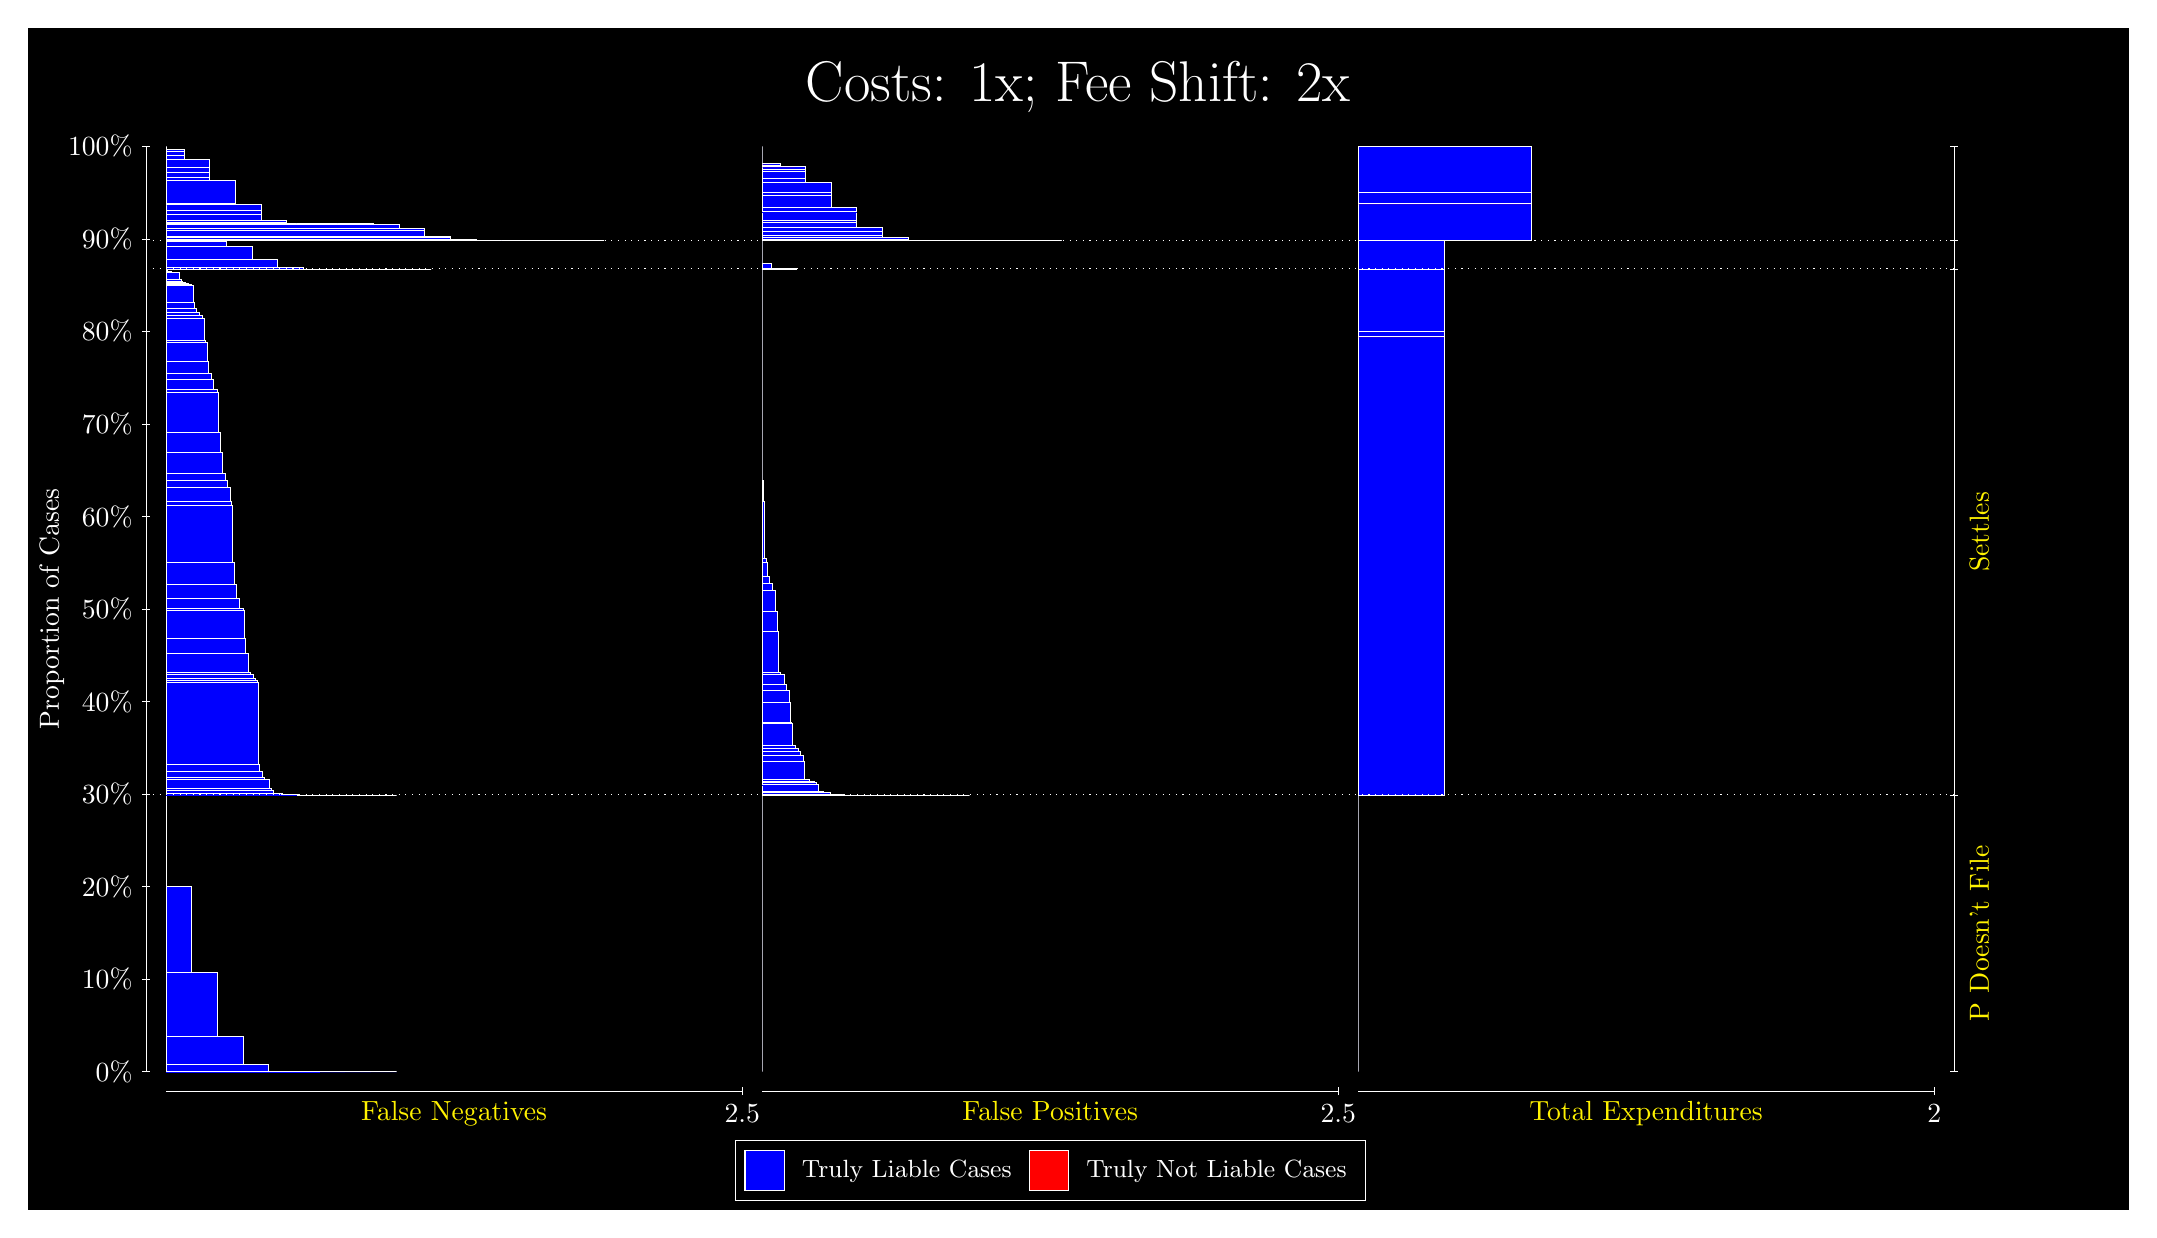
\begin{tikzpicture}
\draw[fill=black] (0,0) rectangle (26.667,15);
\draw[text=white] (0,13.5) rectangle (26.667,15) node[midway] {\huge Costs: 1x; Fee Shift: 2x};
\draw[white, very thin] (1.5,1.75) -- (1.5,13.5);
\node[rotate=90, text=white, anchor=center] at (0.3, 7.625) {Proportion of Cases};
\draw[white, very thin] (1.45,1.75) -- (1.55,1.75);
\node[text=white, anchor=east] at (1.45, 1.75) {0\%};
\draw[white, very thin] (1.45,2.925) -- (1.55,2.925);
\node[text=white, anchor=east] at (1.45, 2.925) {10\%};
\draw[white, very thin] (1.45,4.1) -- (1.55,4.1);
\node[text=white, anchor=east] at (1.45, 4.1) {20\%};
\draw[white, very thin] (1.45,5.275) -- (1.55,5.275);
\node[text=white, anchor=east] at (1.45, 5.275) {30\%};
\draw[white, very thin] (1.45,6.45) -- (1.55,6.45);
\node[text=white, anchor=east] at (1.45, 6.45) {40\%};
\draw[white, very thin] (1.45,7.625) -- (1.55,7.625);
\node[text=white, anchor=east] at (1.45, 7.625) {50\%};
\draw[white, very thin] (1.45,8.8) -- (1.55,8.8);
\node[text=white, anchor=east] at (1.45, 8.8) {60\%};
\draw[white, very thin] (1.45,9.975) -- (1.55,9.975);
\node[text=white, anchor=east] at (1.45, 9.975) {70\%};
\draw[white, very thin] (1.45,11.15) -- (1.55,11.15);
\node[text=white, anchor=east] at (1.45, 11.15) {80\%};
\draw[white, very thin] (1.45,12.325) -- (1.55,12.325);
\node[text=white, anchor=east] at (1.45, 12.325) {90\%};
\draw[white, very thin] (1.45,13.5) -- (1.55,13.5);
\node[text=white, anchor=east] at (1.45, 13.5) {100\%};

\draw[white, very thin] (24.457,1.75) -- (24.457,13.5);
\draw[white, very thin] (24.407,1.75) -- (24.507,1.75);
\node[anchor=west] at (24.407, 1.75) {};
\draw[white, very thin] (24.407,5.264) -- (24.507,5.264);
\node[anchor=west] at (24.407, 5.264) {};
\draw[white, very thin] (24.407,11.943) -- (24.507,11.943);
\node[anchor=west] at (24.407, 11.943) {};
\draw[white, very thin] (24.407,12.305) -- (24.507,12.305);
\node[anchor=west] at (24.407, 12.305) {};
\draw[white, very thin] (24.407,13.5) -- (24.507,13.5);
\node[anchor=west] at (24.407, 13.5) {};

\draw[white, very thin, fill=blue] (1.75,1.75) rectangle (4.6775,1.75);
\draw[white, very thin, fill=blue] (1.75,1.75) rectangle (4.3523,1.75);
\draw[white, very thin, fill=blue] (1.75,1.75) rectangle (4.027,1.75);
\draw[white, very thin, fill=blue] (1.75,1.75) rectangle (3.7017,1.7503);
\draw[white, very thin, fill=blue] (1.75,1.7503) rectangle (3.3764,1.7576);
\draw[white, very thin, fill=blue] (1.75,1.7576) rectangle (3.0511,1.8361);
\draw[white, very thin, fill=blue] (1.75,1.8361) rectangle (2.7258,2.1984);
\draw[white, very thin, fill=blue] (1.75,2.1984) rectangle (2.4006,3.0086);
\draw[white, very thin, fill=blue] (1.75,3.0086) rectangle (2.0753,4.0995);
\draw[white, very thin, fill=red] (1.75,4.0995) rectangle (1.75,4.0995);
\draw[white, very thin, fill=blue] (1.75,4.0995) rectangle (1.75,5.264);
\draw[white, very thin, fill=blue] (1.75,5.264) rectangle (4.6775,5.264);
\draw[white, very thin, fill=blue] (1.75,5.264) rectangle (4.5312,5.264);
\draw[white, very thin, fill=blue] (1.75,5.264) rectangle (4.3848,5.264);
\draw[white, very thin, fill=blue] (1.75,5.264) rectangle (4.3523,5.264);
\draw[white, very thin, fill=blue] (1.75,5.264) rectangle (4.2384,5.264);
\draw[white, very thin, fill=blue] (1.75,5.264) rectangle (4.2059,5.264);
\draw[white, very thin, fill=blue] (1.75,5.264) rectangle (4.092,5.264);
\draw[white, very thin, fill=blue] (1.75,5.264) rectangle (4.0595,5.264);
\draw[white, very thin, fill=blue] (1.75,5.264) rectangle (4.027,5.264);
\draw[white, very thin, fill=blue] (1.75,5.264) rectangle (3.9457,5.264);
\draw[white, very thin, fill=blue] (1.75,5.264) rectangle (3.9131,5.264);
\draw[white, very thin, fill=blue] (1.75,5.264) rectangle (3.8806,5.264);
\draw[white, very thin, fill=blue] (1.75,5.264) rectangle (3.7993,5.264);
\draw[white, very thin, fill=blue] (1.75,5.264) rectangle (3.7668,5.264);
\draw[white, very thin, fill=blue] (1.75,5.264) rectangle (3.7342,5.264);
\draw[white, very thin, fill=blue] (1.75,5.264) rectangle (3.7017,5.264);
\draw[white, very thin, fill=blue] (1.75,5.264) rectangle (3.6529,5.264);
\draw[white, very thin, fill=blue] (1.75,5.264) rectangle (3.6204,5.264);
\draw[white, very thin, fill=blue] (1.75,5.264) rectangle (3.5878,5.2641);
\draw[white, very thin, fill=blue] (1.75,5.2641) rectangle (3.5553,5.2641);
\draw[white, very thin, fill=blue] (1.75,5.2641) rectangle (3.5065,5.2645);
\draw[white, very thin, fill=blue] (1.75,5.2645) rectangle (3.474,5.2645);
\draw[white, very thin, fill=blue] (1.75,5.2645) rectangle (3.4415,5.2654);
\draw[white, very thin, fill=blue] (1.75,5.2654) rectangle (3.4089,5.2659);
\draw[white, very thin, fill=blue] (1.75,5.2659) rectangle (3.3764,5.2661);
\draw[white, very thin, fill=blue] (1.75,5.2661) rectangle (3.3276,5.2668);
\draw[white, very thin, fill=blue] (1.75,5.2668) rectangle (3.2951,5.2712);
\draw[white, very thin, fill=blue] (1.75,5.2712) rectangle (3.2626,5.2763);
\draw[white, very thin, fill=blue] (1.75,5.2763) rectangle (3.23,5.2776);
\draw[white, very thin, fill=blue] (1.75,5.2776) rectangle (3.2138,5.2786);
\draw[white, very thin, fill=blue] (1.75,5.2786) rectangle (3.1812,5.2856);
\draw[white, very thin, fill=blue] (1.75,5.2856) rectangle (3.1487,5.2874);
\draw[white, very thin, fill=blue] (1.75,5.2874) rectangle (3.1162,5.323);
\draw[white, very thin, fill=blue] (1.75,5.323) rectangle (3.0837,5.3484);
\draw[white, very thin, fill=blue] (1.75,5.3484) rectangle (3.0674,5.4605);
\draw[white, very thin, fill=blue] (1.75,5.4605) rectangle (3.0511,5.4655);
\draw[white, very thin, fill=blue] (1.75,5.4655) rectangle (3.0023,5.4879);
\draw[white, very thin, fill=blue] (1.75,5.4879) rectangle (2.9698,5.5574);
\draw[white, very thin, fill=blue] (1.75,5.5574) rectangle (2.9373,5.6463);
\draw[white, very thin, fill=blue] (1.75,5.6463) rectangle (2.921,6.6982);
\draw[white, very thin, fill=blue] (1.75,6.6982) rectangle (2.9048,6.7186);
\draw[white, very thin, fill=blue] (1.75,6.7186) rectangle (2.8885,6.7433);
\draw[white, very thin, fill=blue] (1.75,6.7433) rectangle (2.856,6.7927);
\draw[white, very thin, fill=blue] (1.75,6.7927) rectangle (2.8234,6.8226);
\draw[white, very thin, fill=blue] (1.75,6.8226) rectangle (2.7909,7.0592);
\draw[white, very thin, fill=blue] (1.75,7.0592) rectangle (2.7584,7.2486);
\draw[white, very thin, fill=blue] (1.75,7.2486) rectangle (2.7421,7.602);
\draw[white, very thin, fill=blue] (1.75,7.602) rectangle (2.7258,7.6334);
\draw[white, very thin, fill=blue] (1.75,7.6334) rectangle (2.6771,7.7657);
\draw[white, very thin, fill=blue] (1.75,7.7657) rectangle (2.6445,7.9431);
\draw[white, very thin, fill=blue] (1.75,7.9431) rectangle (2.612,8.2122);
\draw[white, very thin, fill=blue] (1.75,8.2122) rectangle (2.5957,8.9424);
\draw[white, very thin, fill=blue] (1.75,8.9424) rectangle (2.5795,8.9937);
\draw[white, very thin, fill=blue] (1.75,8.9937) rectangle (2.5632,9.1734);
\draw[white, very thin, fill=blue] (1.75,9.1734) rectangle (2.5307,9.261);
\draw[white, very thin, fill=blue] (1.75,9.261) rectangle (2.4982,9.3431);
\draw[white, very thin, fill=blue] (1.75,9.3431) rectangle (2.4656,9.6089);
\draw[white, very thin, fill=blue] (1.75,9.6089) rectangle (2.4331,9.8712);
\draw[white, very thin, fill=blue] (1.75,9.8712) rectangle (2.4168,10.38);
\draw[white, very thin, fill=blue] (1.75,10.38) rectangle (2.4006,10.412);
\draw[white, very thin, fill=blue] (1.75,10.412) rectangle (2.3518,10.543);
\draw[white, very thin, fill=blue] (1.75,10.543) rectangle (2.3192,10.617);
\draw[white, very thin, fill=blue] (1.75,10.617) rectangle (2.2867,10.77);
\draw[white, very thin, fill=blue] (1.75,10.77) rectangle (2.2705,11.017);
\draw[white, very thin, fill=blue] (1.75,11.017) rectangle (2.2542,11.037);
\draw[white, very thin, fill=blue] (1.75,11.037) rectangle (2.2379,11.319);
\draw[white, very thin, fill=blue] (1.75,11.319) rectangle (2.2054,11.349);
\draw[white, very thin, fill=blue] (1.75,11.349) rectangle (2.1729,11.389);
\draw[white, very thin, fill=blue] (1.75,11.389) rectangle (2.1403,11.442);
\draw[white, very thin, fill=blue] (1.75,11.442) rectangle (2.1078,11.514);
\draw[white, very thin, fill=blue] (1.75,11.514) rectangle (2.0915,11.74);
\draw[white, very thin, fill=blue] (1.75,11.74) rectangle (2.0753,11.746);
\draw[white, very thin, fill=blue] (1.75,11.746) rectangle (2.0265,11.767);
\draw[white, very thin, fill=blue] (1.75,11.767) rectangle (1.994,11.772);
\draw[white, very thin, fill=blue] (1.75,11.772) rectangle (1.9614,11.789);
\draw[white, very thin, fill=blue] (1.75,11.789) rectangle (1.9452,11.813);
\draw[white, very thin, fill=blue] (1.75,11.813) rectangle (1.9289,11.815);
\draw[white, very thin, fill=blue] (1.75,11.815) rectangle (1.9126,11.901);
\draw[white, very thin, fill=blue] (1.75,11.901) rectangle (1.8801,11.903);
\draw[white, very thin, fill=blue] (1.75,11.903) rectangle (1.8476,11.906);
\draw[white, very thin, fill=blue] (1.75,11.906) rectangle (1.8151,11.908);
\draw[white, very thin, fill=blue] (1.75,11.908) rectangle (1.7825,11.912);
\draw[white, very thin, fill=blue] (1.75,11.912) rectangle (1.7663,11.936);
\draw[white, very thin, fill=red] (1.75,11.936) rectangle (1.75,11.936);
\draw[white, very thin, fill=blue] (1.75,11.936) rectangle (1.75,11.943);
\draw[white, very thin, fill=blue] (1.75,11.943) rectangle (5.1167,11.943);
\draw[white, very thin, fill=blue] (1.75,11.943) rectangle (4.7914,11.943);
\draw[white, very thin, fill=blue] (1.75,11.943) rectangle (4.4661,11.943);
\draw[white, very thin, fill=blue] (1.75,11.943) rectangle (4.1408,11.943);
\draw[white, very thin, fill=blue] (1.75,11.943) rectangle (3.8155,11.944);
\draw[white, very thin, fill=blue] (1.75,11.944) rectangle (3.4903,11.958);
\draw[white, very thin, fill=blue] (1.75,11.958) rectangle (3.165,12.065);
\draw[white, very thin, fill=blue] (1.75,12.065) rectangle (2.8397,12.23);
\draw[white, very thin, fill=blue] (1.75,12.23) rectangle (2.5144,12.295);
\draw[white, very thin, fill=blue] (1.75,12.295) rectangle (2.1891,12.305);
\draw[white, very thin, fill=red] (1.75,12.305) rectangle (1.75,12.305);
\draw[white, very thin, fill=blue] (1.75,12.305) rectangle (7.3123,12.305);
\draw[white, very thin, fill=blue] (1.75,12.305) rectangle (6.9871,12.305);
\draw[white, very thin, fill=blue] (1.75,12.305) rectangle (6.6618,12.305);
\draw[white, very thin, fill=blue] (1.75,12.305) rectangle (6.3365,12.305);
\draw[white, very thin, fill=blue] (1.75,12.305) rectangle (6.3365,12.305);
\draw[white, very thin, fill=blue] (1.75,12.305) rectangle (6.0112,12.306);
\draw[white, very thin, fill=blue] (1.75,12.306) rectangle (6.0112,12.306);
\draw[white, very thin, fill=blue] (1.75,12.306) rectangle (5.6859,12.308);
\draw[white, very thin, fill=blue] (1.75,12.308) rectangle (5.6859,12.315);
\draw[white, very thin, fill=blue] (1.75,12.315) rectangle (5.3606,12.342);
\draw[white, very thin, fill=blue] (1.75,12.342) rectangle (5.3606,12.357);
\draw[white, very thin, fill=blue] (1.75,12.357) rectangle (5.2305,12.357);
\draw[white, very thin, fill=blue] (1.75,12.357) rectangle (5.0354,12.44);
\draw[white, very thin, fill=blue] (1.75,12.44) rectangle (5.0354,12.453);
\draw[white, very thin, fill=blue] (1.75,12.453) rectangle (4.9052,12.453);
\draw[white, very thin, fill=blue] (1.75,12.453) rectangle (4.7101,12.515);
\draw[white, very thin, fill=blue] (1.75,12.515) rectangle (4.58,12.515);
\draw[white, very thin, fill=blue] (1.75,12.515) rectangle (4.58,12.515);
\draw[white, very thin, fill=blue] (1.75,12.515) rectangle (4.3848,12.522);
\draw[white, very thin, fill=blue] (1.75,12.522) rectangle (4.2547,12.522);
\draw[white, very thin, fill=blue] (1.75,12.522) rectangle (4.2547,12.522);
\draw[white, very thin, fill=blue] (1.75,12.522) rectangle (4.0595,12.522);
\draw[white, very thin, fill=blue] (1.75,12.522) rectangle (4.0595,12.522);
\draw[white, very thin, fill=blue] (1.75,12.522) rectangle (3.9294,12.522);
\draw[white, very thin, fill=blue] (1.75,12.522) rectangle (3.7342,12.522);
\draw[white, very thin, fill=blue] (1.75,12.522) rectangle (3.7342,12.522);
\draw[white, very thin, fill=blue] (1.75,12.522) rectangle (3.7342,12.522);
\draw[white, very thin, fill=blue] (1.75,12.522) rectangle (3.6041,12.524);
\draw[white, very thin, fill=blue] (1.75,12.524) rectangle (3.4089,12.524);
\draw[white, very thin, fill=blue] (1.75,12.524) rectangle (3.4089,12.524);
\draw[white, very thin, fill=blue] (1.75,12.524) rectangle (3.2788,12.53);
\draw[white, very thin, fill=blue] (1.75,12.53) rectangle (3.2788,12.564);
\draw[white, very thin, fill=blue] (1.75,12.564) rectangle (3.0837,12.564);
\draw[white, very thin, fill=blue] (1.75,12.564) rectangle (3.0837,12.564);
\draw[white, very thin, fill=blue] (1.75,12.564) rectangle (2.9535,12.567);
\draw[white, very thin, fill=blue] (1.75,12.567) rectangle (2.9535,12.633);
\draw[white, very thin, fill=blue] (1.75,12.633) rectangle (2.9535,12.692);
\draw[white, very thin, fill=blue] (1.75,12.692) rectangle (2.9535,12.76);
\draw[white, very thin, fill=blue] (1.75,12.76) rectangle (2.7584,12.76);
\draw[white, very thin, fill=blue] (1.75,12.76) rectangle (2.6283,12.783);
\draw[white, very thin, fill=blue] (1.75,12.783) rectangle (2.6283,13.074);
\draw[white, very thin, fill=blue] (1.75,13.074) rectangle (2.303,13.11);
\draw[white, very thin, fill=blue] (1.75,13.11) rectangle (2.303,13.17);
\draw[white, very thin, fill=blue] (1.75,13.17) rectangle (2.303,13.229);
\draw[white, very thin, fill=blue] (1.75,13.229) rectangle (2.303,13.33);
\draw[white, very thin, fill=blue] (1.75,13.33) rectangle (1.9777,13.38);
\draw[white, very thin, fill=blue] (1.75,13.38) rectangle (1.9777,13.44);
\draw[white, very thin, fill=blue] (1.75,13.44) rectangle (1.9777,13.457);
\draw[white, very thin, fill=red] (1.75,13.457) rectangle (1.75,13.457);
\draw[white, very thin, fill=blue] (1.75,13.457) rectangle (1.75,13.5);
\draw[white, very thin, fill=red] (9.3189,1.75) rectangle (9.3189,1.75);
\draw[white, very thin, fill=blue] (9.3189,1.75) rectangle (9.3189,5.264);
\draw[white, very thin, fill=red] (9.3189,5.264) rectangle (11.954,5.264);
\draw[white, very thin, fill=blue] (9.3189,5.264) rectangle (11.954,5.264);
\draw[white, very thin, fill=red] (9.3189,5.264) rectangle (11.807,5.264);
\draw[white, very thin, fill=blue] (9.3189,5.264) rectangle (11.807,5.264);
\draw[white, very thin, fill=red] (9.3189,5.264) rectangle (11.661,5.264);
\draw[white, very thin, fill=blue] (9.3189,5.264) rectangle (11.661,5.264);
\draw[white, very thin, fill=blue] (9.3189,5.264) rectangle (11.628,5.264);
\draw[white, very thin, fill=blue] (9.3189,5.264) rectangle (11.482,5.264);
\draw[white, very thin, fill=red] (9.3189,5.264) rectangle (11.368,5.264);
\draw[white, very thin, fill=blue] (9.3189,5.264) rectangle (11.368,5.264);
\draw[white, very thin, fill=blue] (9.3189,5.264) rectangle (11.336,5.264);
\draw[white, very thin, fill=blue] (9.3189,5.264) rectangle (11.303,5.264);
\draw[white, very thin, fill=red] (9.3189,5.264) rectangle (11.222,5.264);
\draw[white, very thin, fill=blue] (9.3189,5.264) rectangle (11.222,5.264);
\draw[white, very thin, fill=blue] (9.3189,5.264) rectangle (11.157,5.264);
\draw[white, very thin, fill=red] (9.3189,5.264) rectangle (11.075,5.264);
\draw[white, very thin, fill=blue] (9.3189,5.264) rectangle (11.075,5.264);
\draw[white, very thin, fill=blue] (9.3189,5.264) rectangle (11.043,5.264);
\draw[white, very thin, fill=blue] (9.3189,5.264) rectangle (11.01,5.264);
\draw[white, very thin, fill=blue] (9.3189,5.264) rectangle (10.978,5.264);
\draw[white, very thin, fill=red] (9.3189,5.264) rectangle (10.929,5.264);
\draw[white, very thin, fill=blue] (9.3189,5.264) rectangle (10.929,5.264);
\draw[white, very thin, fill=blue] (9.3189,5.264) rectangle (10.896,5.264);
\draw[white, very thin, fill=blue] (9.3189,5.264) rectangle (10.831,5.264);
\draw[white, very thin, fill=red] (9.3189,5.264) rectangle (10.783,5.264);
\draw[white, very thin, fill=blue] (9.3189,5.264) rectangle (10.783,5.264);
\draw[white, very thin, fill=blue] (9.3189,5.264) rectangle (10.75,5.264);
\draw[white, very thin, fill=blue] (9.3189,5.264) rectangle (10.718,5.264);
\draw[white, very thin, fill=blue] (9.3189,5.264) rectangle (10.685,5.264);
\draw[white, very thin, fill=blue] (9.3189,5.264) rectangle (10.653,5.264);
\draw[white, very thin, fill=red] (9.3189,5.264) rectangle (10.636,5.264);
\draw[white, very thin, fill=blue] (9.3189,5.264) rectangle (10.636,5.264);
\draw[white, very thin, fill=blue] (9.3189,5.264) rectangle (10.604,5.264);
\draw[white, very thin, fill=blue] (9.3189,5.264) rectangle (10.571,5.264);
\draw[white, very thin, fill=blue] (9.3189,5.264) rectangle (10.506,5.2645);
\draw[white, very thin, fill=red] (9.3189,5.2645) rectangle (10.49,5.2645);
\draw[white, very thin, fill=blue] (9.3189,5.2645) rectangle (10.49,5.2646);
\draw[white, very thin, fill=blue] (9.3189,5.2646) rectangle (10.457,5.2646);
\draw[white, very thin, fill=blue] (9.3189,5.2646) rectangle (10.425,5.2646);
\draw[white, very thin, fill=blue] (9.3189,5.2646) rectangle (10.392,5.2647);
\draw[white, very thin, fill=blue] (9.3189,5.2647) rectangle (10.36,5.2694);
\draw[white, very thin, fill=red] (9.3189,5.2694) rectangle (10.344,5.2694);
\draw[white, very thin, fill=blue] (9.3189,5.2694) rectangle (10.344,5.2694);
\draw[white, very thin, fill=blue] (9.3189,5.2694) rectangle (10.327,5.2699);
\draw[white, very thin, fill=blue] (9.3189,5.2699) rectangle (10.311,5.2703);
\draw[white, very thin, fill=blue] (9.3189,5.2703) rectangle (10.278,5.2704);
\draw[white, very thin, fill=blue] (9.3189,5.2704) rectangle (10.246,5.2709);
\draw[white, very thin, fill=red] (9.3189,5.2709) rectangle (10.197,5.2709);
\draw[white, very thin, fill=blue] (9.3189,5.2709) rectangle (10.197,5.2712);
\draw[white, very thin, fill=blue] (9.3189,5.2712) rectangle (10.181,5.2949);
\draw[white, very thin, fill=blue] (9.3189,5.2949) rectangle (10.165,5.299);
\draw[white, very thin, fill=blue] (9.3189,5.299) rectangle (10.132,5.3011);
\draw[white, very thin, fill=blue] (9.3189,5.3011) rectangle (10.1,5.3047);
\draw[white, very thin, fill=blue] (9.3189,5.3047) rectangle (10.067,5.3065);
\draw[white, very thin, fill=blue] (9.3189,5.3065) rectangle (10.034,5.3924);
\draw[white, very thin, fill=blue] (9.3189,5.3924) rectangle (10.018,5.3938);
\draw[white, very thin, fill=blue] (9.3189,5.3938) rectangle (10.002,5.418);
\draw[white, very thin, fill=blue] (9.3189,5.418) rectangle (9.9857,5.4351);
\draw[white, very thin, fill=blue] (9.3189,5.4351) rectangle (9.9532,5.4402);
\draw[white, very thin, fill=blue] (9.3189,5.4402) rectangle (9.9206,5.4615);
\draw[white, very thin, fill=blue] (9.3189,5.4615) rectangle (9.8718,5.4672);
\draw[white, very thin, fill=blue] (9.3189,5.4672) rectangle (9.8556,5.6935);
\draw[white, very thin, fill=blue] (9.3189,5.6935) rectangle (9.8393,5.765);
\draw[white, very thin, fill=blue] (9.3189,5.765) rectangle (9.8068,5.8186);
\draw[white, very thin, fill=blue] (9.3189,5.8186) rectangle (9.7743,5.8585);
\draw[white, very thin, fill=blue] (9.3189,5.8585) rectangle (9.7417,5.8886);
\draw[white, very thin, fill=blue] (9.3189,5.8886) rectangle (9.7092,6.1698);
\draw[white, very thin, fill=blue] (9.3189,6.1698) rectangle (9.6929,6.1904);
\draw[white, very thin, fill=blue] (9.3189,6.1904) rectangle (9.6767,6.4369);
\draw[white, very thin, fill=blue] (9.3189,6.4369) rectangle (9.6604,6.5902);
\draw[white, very thin, fill=blue] (9.3189,6.5902) rectangle (9.6279,6.6639);
\draw[white, very thin, fill=blue] (9.3189,6.6639) rectangle (9.5954,6.795);
\draw[white, very thin, fill=blue] (9.3189,6.795) rectangle (9.5466,6.8268);
\draw[white, very thin, fill=blue] (9.3189,6.8268) rectangle (9.5303,7.3361);
\draw[white, very thin, fill=blue] (9.3189,7.3361) rectangle (9.514,7.5983);
\draw[white, very thin, fill=blue] (9.3189,7.5983) rectangle (9.4815,7.8641);
\draw[white, very thin, fill=blue] (9.3189,7.8641) rectangle (9.449,7.9463);
\draw[white, very thin, fill=blue] (9.3189,7.9463) rectangle (9.4165,8.0339);
\draw[white, very thin, fill=blue] (9.3189,8.0339) rectangle (9.3839,8.2135);
\draw[white, very thin, fill=blue] (9.3189,8.2135) rectangle (9.3677,8.2648);
\draw[white, very thin, fill=blue] (9.3189,8.2648) rectangle (9.3514,8.995);
\draw[white, very thin, fill=blue] (9.3189,8.995) rectangle (9.3351,9.2641);
\draw[white, very thin, fill=blue] (9.3189,9.2641) rectangle (9.3189,11.943);
\draw[white, very thin, fill=red] (9.3189,11.943) rectangle (9.758,11.943);
\draw[white, very thin, fill=blue] (9.3189,11.943) rectangle (9.758,11.953);
\draw[white, very thin, fill=blue] (9.3189,11.953) rectangle (9.4327,12.018);
\draw[white, very thin, fill=blue] (9.3189,12.018) rectangle (9.3189,12.305);
\draw[white, very thin, fill=red] (9.3189,12.305) rectangle (13.125,12.305);
\draw[white, very thin, fill=blue] (9.3189,12.305) rectangle (13.125,12.305);
\draw[white, very thin, fill=red] (9.3189,12.305) rectangle (12.799,12.305);
\draw[white, very thin, fill=blue] (9.3189,12.305) rectangle (12.799,12.305);
\draw[white, very thin, fill=blue] (9.3189,12.305) rectangle (12.474,12.305);
\draw[white, very thin, fill=red] (9.3189,12.305) rectangle (12.474,12.305);
\draw[white, very thin, fill=blue] (9.3189,12.305) rectangle (12.474,12.305);
\draw[white, very thin, fill=blue] (9.3189,12.305) rectangle (12.149,12.305);
\draw[white, very thin, fill=blue] (9.3189,12.305) rectangle (12.149,12.305);
\draw[white, very thin, fill=red] (9.3189,12.305) rectangle (12.149,12.305);
\draw[white, very thin, fill=blue] (9.3189,12.305) rectangle (12.149,12.305);
\draw[white, very thin, fill=red] (9.3189,12.305) rectangle (11.824,12.305);
\draw[white, very thin, fill=blue] (9.3189,12.305) rectangle (11.824,12.306);
\draw[white, very thin, fill=blue] (9.3189,12.306) rectangle (11.824,12.306);
\draw[white, very thin, fill=blue] (9.3189,12.306) rectangle (11.824,12.306);
\draw[white, very thin, fill=red] (9.3189,12.306) rectangle (11.498,12.306);
\draw[white, very thin, fill=blue] (9.3189,12.306) rectangle (11.498,12.311);
\draw[white, very thin, fill=blue] (9.3189,12.311) rectangle (11.498,12.312);
\draw[white, very thin, fill=blue] (9.3189,12.312) rectangle (11.173,12.325);
\draw[white, very thin, fill=red] (9.3189,12.325) rectangle (11.173,12.325);
\draw[white, very thin, fill=blue] (9.3189,12.325) rectangle (11.173,12.349);
\draw[white, very thin, fill=blue] (9.3189,12.349) rectangle (10.848,12.365);
\draw[white, very thin, fill=blue] (9.3189,12.365) rectangle (10.848,12.422);
\draw[white, very thin, fill=red] (9.3189,12.422) rectangle (10.848,12.422);
\draw[white, very thin, fill=blue] (9.3189,12.422) rectangle (10.848,12.475);
\draw[white, very thin, fill=blue] (9.3189,12.475) rectangle (10.522,12.53);
\draw[white, very thin, fill=blue] (9.3189,12.53) rectangle (10.522,12.561);
\draw[white, very thin, fill=red] (9.3189,12.561) rectangle (10.522,12.561);
\draw[white, very thin, fill=blue] (9.3189,12.561) rectangle (10.522,12.669);
\draw[white, very thin, fill=blue] (9.3189,12.669) rectangle (10.522,12.671);
\draw[white, very thin, fill=blue] (9.3189,12.671) rectangle (10.522,12.731);
\draw[white, very thin, fill=blue] (9.3189,12.731) rectangle (10.197,12.872);
\draw[white, very thin, fill=blue] (9.3189,12.872) rectangle (10.197,12.911);
\draw[white, very thin, fill=blue] (9.3189,12.911) rectangle (10.197,13.045);
\draw[white, very thin, fill=red] (9.3189,13.045) rectangle (10.067,13.045);
\draw[white, very thin, fill=blue] (9.3189,13.045) rectangle (10.067,13.045);
\draw[white, very thin, fill=blue] (9.3189,13.045) rectangle (9.8718,13.099);
\draw[white, very thin, fill=blue] (9.3189,13.099) rectangle (9.8718,13.182);
\draw[white, very thin, fill=blue] (9.3189,13.182) rectangle (9.8718,13.206);
\draw[white, very thin, fill=blue] (9.3189,13.206) rectangle (9.8718,13.242);
\draw[white, very thin, fill=blue] (9.3189,13.242) rectangle (9.7417,13.242);
\draw[white, very thin, fill=red] (9.3189,13.242) rectangle (9.7417,13.242);
\draw[white, very thin, fill=blue] (9.3189,13.242) rectangle (9.7417,13.242);
\draw[white, very thin, fill=blue] (9.3189,13.242) rectangle (9.5466,13.256);
\draw[white, very thin, fill=blue] (9.3189,13.256) rectangle (9.5466,13.259);
\draw[white, very thin, fill=blue] (9.3189,13.259) rectangle (9.5466,13.281);
\draw[white, very thin, fill=blue] (9.3189,13.281) rectangle (9.4165,13.281);
\draw[white, very thin, fill=red] (9.3189,13.281) rectangle (9.4165,13.281);
\draw[white, very thin, fill=blue] (9.3189,13.281) rectangle (9.4165,13.281);
\draw[white, very thin, fill=red] (9.3189,13.281) rectangle (9.3189,13.281);
\draw[white, very thin, fill=blue] (9.3189,13.281) rectangle (9.3189,13.5);
\draw[white, very thin, fill=red] (16.888,1.75) rectangle (16.888,1.75);
\draw[white, very thin, fill=blue] (16.888,1.75) rectangle (16.888,5.264);
\draw[white, very thin, fill=red] (16.888,5.264) rectangle (17.986,5.264);
\draw[white, very thin, fill=blue] (16.888,5.264) rectangle (17.986,11.083);
\draw[white, very thin, fill=red] (16.888,11.083) rectangle (17.986,11.083);
\draw[white, very thin, fill=blue] (16.888,11.083) rectangle (17.986,11.157);
\draw[white, very thin, fill=red] (16.888,11.157) rectangle (17.986,11.157);
\draw[white, very thin, fill=blue] (16.888,11.157) rectangle (17.986,11.943);
\draw[white, very thin, fill=red] (16.888,11.943) rectangle (17.986,11.943);
\draw[white, very thin, fill=blue] (16.888,11.943) rectangle (17.986,12.305);
\draw[white, very thin, fill=red] (16.888,12.305) rectangle (19.083,12.305);
\draw[white, very thin, fill=blue] (16.888,12.305) rectangle (19.083,12.772);
\draw[white, very thin, fill=red] (16.888,12.772) rectangle (19.083,12.772);
\draw[white, very thin, fill=blue] (16.888,12.772) rectangle (19.083,12.918);
\draw[white, very thin, fill=red] (16.888,12.918) rectangle (19.083,12.918);
\draw[white, very thin, fill=blue] (16.888,12.918) rectangle (19.083,13.5);
\draw[white, dotted] (1.5,5.264) -- (24.457,5.264);
\draw[white, dotted] (1.5,11.943) -- (24.457,11.943);
\draw[white, dotted] (1.5,12.305) -- (24.457,12.305);
\draw[white, very thin] (1.75,1.5) -- (9.0689,1.5);
\node[text=yellow, anchor=north] at (5.4094, 1.5) {False Negatives};
\draw[white, very thin] (9.0689,1.45) -- (9.0689,1.55);
\node[text=white, anchor=north] at (9.0689, 1.45) {2.5};

\draw[white, very thin] (9.3189,1.5) -- (16.638,1.5);
\node[text=yellow, anchor=north] at (12.978, 1.5) {False Positives};
\draw[white, very thin] (16.638,1.45) -- (16.638,1.55);
\node[text=white, anchor=north] at (16.638, 1.45) {2.5};

\draw[white, very thin] (16.888,1.5) -- (24.207,1.5);
\node[text=yellow, anchor=north] at (20.547, 1.5) {Total Expenditures};
\draw[white, very thin] (24.207,1.45) -- (24.207,1.55);
\node[text=white, anchor=north] at (24.207, 1.45) {2};

\node[text=yellow, centered, rotate=90] at (24.777, 3.507) {P Doesn't File};
\node[text=yellow, centered, rotate=90] at (24.777, 8.6036) {Settles};



\draw (12.978300999999998,1.5) node[draw=none] (baseCoordinate) {};
\begin{scope}[align=center]
        \matrix[scale=0.5, draw=white, below=0.5cm of baseCoordinate, nodes={draw}, column sep=0.1cm]{
            \node[rectangle, draw, minimum width=0.5cm, minimum height=0.5cm, fill=blue] {}; &
            \node[draw=none, font=\small, text=white] (B) {Truly Liable Cases}; &
            \node[rectangle, draw, minimum width=0.5cm, minimum height=0.5cm, fill=red] {}; &
            \node[draw=none, font=\small, text=white] (B) {Truly Not Liable Cases}; \\
            };
\end{scope}

\end{tikzpicture}
\end{document}